
\chapter{Quark Gluon Analysis}
\label{ch:quark_gluon_analysis}

\section{Sidenotes}\label{sec:sidenotes}
One of the most prominent and distinctive features of this style is the
extensive use of sidenotes.  There is a wide margin to provide ample room
for sidenotes and small figures.  Any \doccmd{footnote}s will automatically
be converted to sidenotes.\footnote{This is a sidenote that was entered
using the \texttt{\textbackslash footnote} command.}  If you'd like to place ancillary
information in the margin without the sidenote mark (the superscript
number), you can use the \doccmd{marginnote} command.\marginnote{This is a
margin note.  Notice that there isn't a number preceding the note, and
there is no number in the main text where this note was written.}





\begin{figure}
  \includegraphics[width=0.95\textwidth, trim=0 0 0 0, clip]{figures/quarks/btagging_variables_hist-down_sample=1.00-ML_vars=vertex-selection=b-ejet_min=4-n_iter_RS_lgb=99-n_iter_RS_xgb=9-cdot_cut=0.90-version=19.pdf}
  \caption[Histograms of the vertex variables]
          {Histograms of the three vertex variables, \code{projet}, \code{bqvjet}, and \code{ptljet}, used as input variables in the b-tagging models. In blue colors the variables are shown for \textcolor{blue}{true b-jets}, in red for \textcolor{red}{true c-jets}, in green for \textcolor{green}{true g-jets}, and in orange for \textcolor{orange}{all of the jets} (including non q-matched). In fully opaque color are shown the distributions for 2-jet events, in dashed (and lighter color) 3-jet events, and in semi-transparent 4-jet events. Notice the logarithmic y-axis, that there are no g-jets for 2-jet events (as expected), and that all of the distributions are very similar not matter how many jets.
          } 
  \label{fig:q:vertex_variables}
\end{figure}



\begin{figure}
  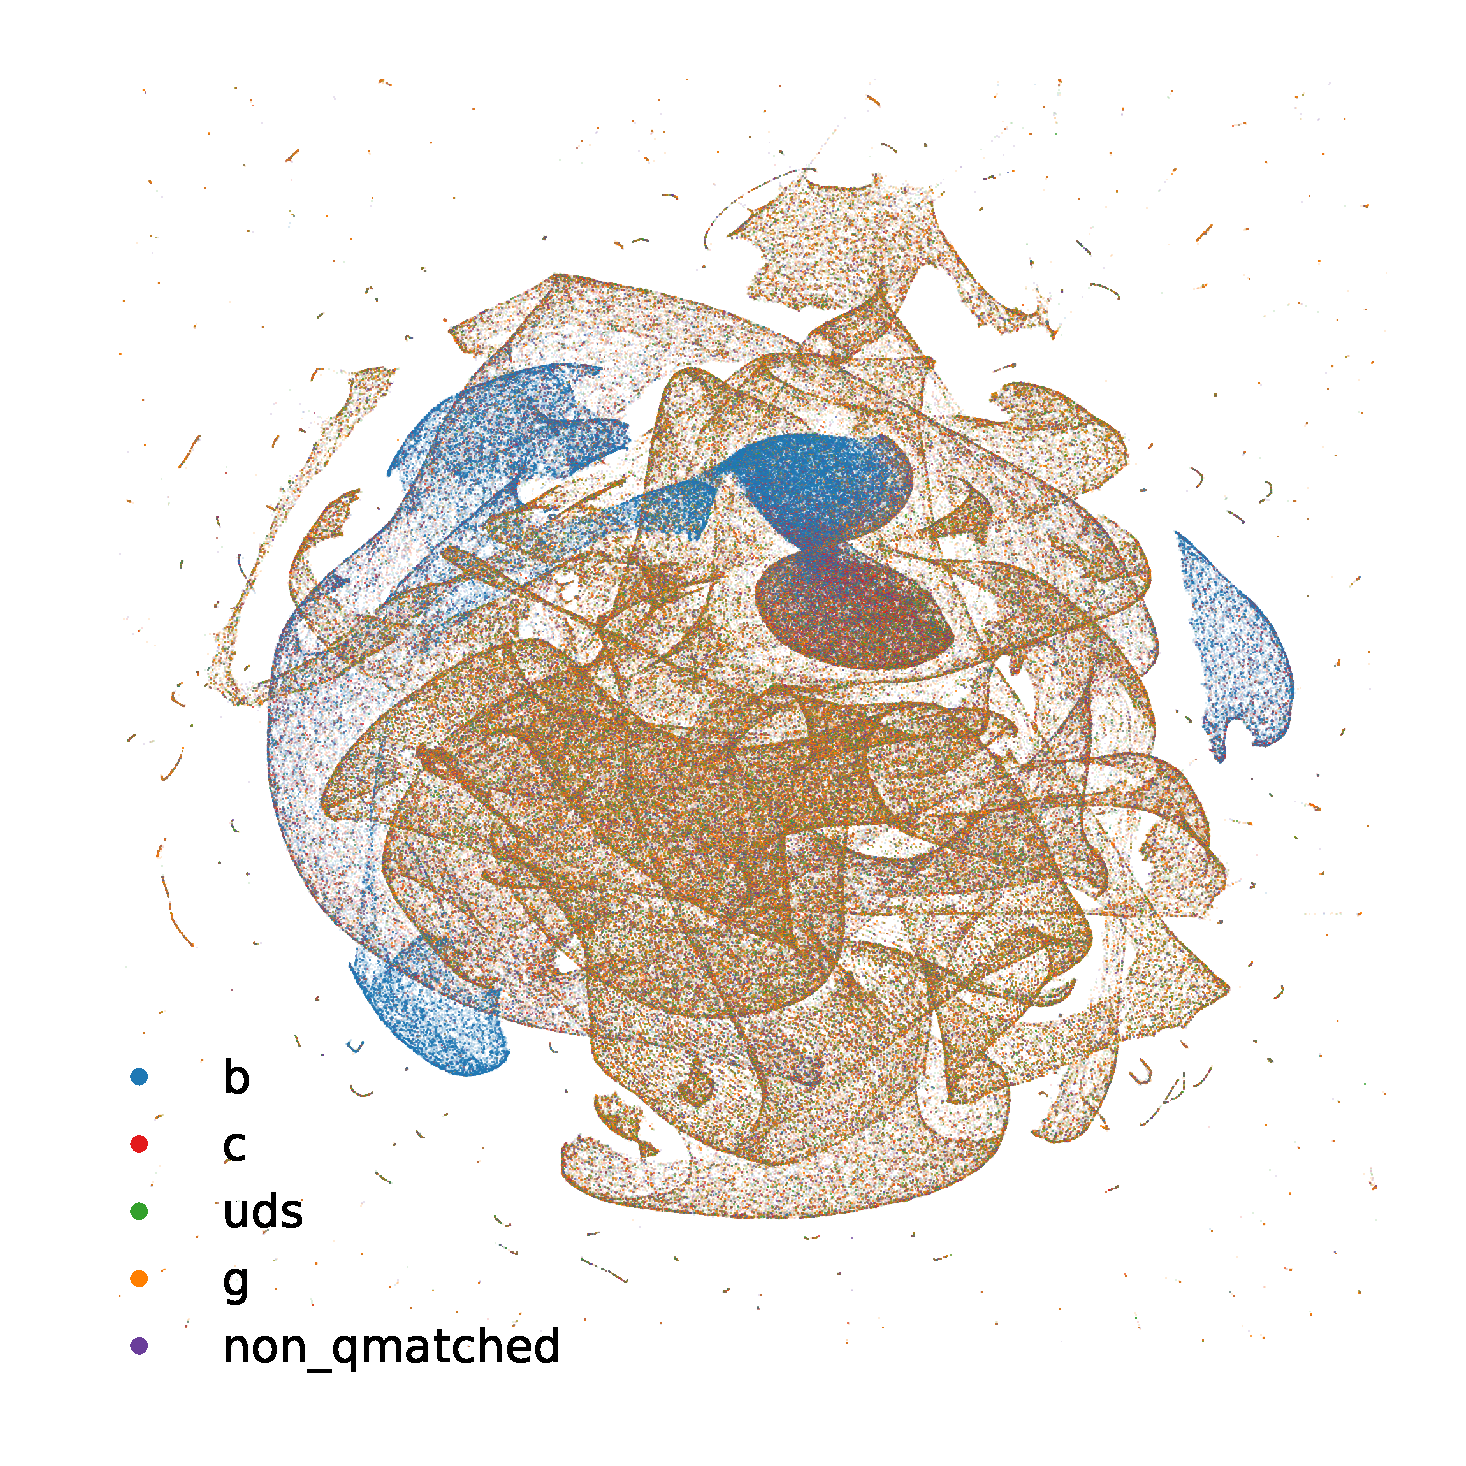
\includegraphics[width=0.95\textwidth, trim=20 20 50 50, clip]{figures/quarks/df_UMAP-X=1120952-n_neighbors=250-min_dist=0.2-metric=euclidean-input2b_njet=4_algorithm=UMAP_single.pdf}
  \caption[UMAP vizualisation of vertex variables]
          {Vizualisation of the vertex variables for the different categories: \textcolor{blue}{true b-jets} in blue, \textcolor{red}{true c-jets} in red, \textcolor{green}{true uds-jets} in green, \textcolor{orange}{true g-jets} in orange, and \textcolor{purple}{non q-matched}. The clustering is performed with the UMAP algorithm which outputs a 2D-projection. This projection is then visualized using the Datashader which takes takes care of point size, avoids over- and under-plotting, and color intensity. 
          } 
  \label{fig:q:UMAP_vertex}
\end{figure}



\begin{figure}
  \includegraphics[width=0.95\textwidth, trim=0 0 0 30, clip]{figures/quarks/y_pred_3_jet_hist-down_sample=1.00-ML_vars=vertex-selection=b-ejet_min=4-n_iter_RS_lgb=99-n_iter_RS_xgb=9-cdot_cut=0.90-version=19.pdf}
  \caption[b-tag scores in 3-jet events]
          {Histogram of b-tag scores (model prediction) in 3-jet events for \textcolor{blue}{NNB} (the neural network trained by ATLAS, also called \code{nnbjet}) in blue, \textcolor{red}{XGB} in red, and \textcolor{green}{XGB} in green. We see that the XGB predictions closely match those of NNB which is a good confirmation of a successful fit.  
          } 
  \label{fig:q:btag_scores_3j}
\end{figure}




\begin{figure}
  \includegraphics[width=0.95\textwidth, trim=10 10 10 40, clip]{figures/quarks/ROC_4_jet-down_sample=1.00-ML_vars=vertex-selection=b-ejet_min=4-n_iter_RS_lgb=99-n_iter_RS_xgb=9-cdot_cut=0.90-version=19.pdf}
  \caption[ROC curve for b-tag in 4-jet events]
          {ROC curve of the three b-tag models in 3-jet events for \textcolor{blue}{NNB} (the neural network trained by ATLAS, also called \code{nnbjet}) in blue, \textcolor{red}{XGB} in red, and \textcolor{green}{XGB} in green. In the legend the Area Under Curve (AUC) is also shown. Notice that the XGB and XGB models share performance and it is thus due to overplotting that only the green line for XGB can be seen. In the particle physics community False Positive Rate (FPR) is sometimes better known as background efficiency and True Positive Rate (TPR) as signal efficiency.  
          } 
  \label{fig:q:roc_btag_4j}
\end{figure}




\begin{figure}
  \includegraphics[width=0.95\textwidth, trim=10 10 10 40, clip]{figures/quarks/gtag_y_pred_4_jet_hist-down_sample=1.00-ML_vars=vertex-selection=b-ejet_min=4-n_iter_RS_lgb=99-n_iter_RS_xgb=9-cdot_cut=0.90-version=19.pdf}
  \caption[g-tag scores in 4-jet events]
          {
            Histogram of g-tag scores (model prediction) in 4-jet events for \textcolor{blue}{XGB: Energy Ordered} in blue, \textcolor{red}{XGB: Shuffled} in red, \textcolor{green}{XGB: All Permutations} in green, \textcolor{orange}{XGB: Sum 1D} in orange, \textcolor{purple}{PermNet: Energy Ordered} in purple, \textcolor{light-blue}{PermNet: Shuffled} in light-blue, \textcolor{light-green}{PermNet: All Permutations} in light-green, \textcolor{light-purple}{PermNet: Sum 1D} in light-purple.  Here XGB and PermNet are the two different type of models and \q{Energy Ordered}, \q{Shuffled}, \q{All Permutations}, and \q{Sum 1D} are the different methods used for making the input data permutation invariant.  
          }   
  \label{fig:q:gtag_scores_4j}
\end{figure}


\begin{figure}
  \includegraphics[width=0.95\textwidth, trim=10 10 10 40, clip]{figures/quarks/gtag-histogram-sigbkg-down_sample=1.00-ML_vars=vertex-selection=b-ejet_min=4-n_iter_RS_lgb=99-n_iter_RS_xgb=9-cdot_cut=0.90-version=19-njet=4.pdf}
  \caption[g-tag scores in 4-jet events for signal and background]
          {Histogram of g-tag scores (model prediction) from the XGB-model in 4-jet events for \textcolor{blue}{b signal} in blue, \textcolor{red}{c signal} in red, \textcolor{green}{l signal} in green, \textcolor{orange}{b background} in orange, \textcolor{purple}{c background} in purple, \textcolor{light-blue}{l background} in light-blue.
          } 
  \label{fig:q:gtag_scores_4j_sig_bkg}
\end{figure}





\begin{figure}
  \includegraphics[width=0.95\textwidth, trim=10 10 10 40, clip]{figures/quarks/gtag_ROC_4_jet-down_sample=1.00-ML_vars=vertex-selection=b-ejet_min=4-n_iter_RS_lgb=99-n_iter_RS_xgb=9-cdot_cut=0.90-version=19.pdf}
  \caption[ROC curve for g-tag in 4-jet events]
          {ROC curve of the eight g-tag models in 4-jet events. First one in dashed black is the ROC curve that you get by random chance. The colors are the same as in \figref{fig:q:gtag_scores_4j} and in the legend also the Area Under the ROC curve (AUC) is shown. 
          Notice that the XGB model which uses the energy ordered data produced the best model, however, this model is not permutation invariant. Of the permutation invariant models (the rest), the XGB model trained on all permutations of the b-tags performs highest. The lowest performing models are the two models trained only on the 1-dimensional sum of b-tags, as expected, however, still with a better performance than expected by the author.  
          } 
  \label{fig:q:roc_gtag_4j}
\end{figure}





\begin{figure}
  \includegraphics[width=0.95\textwidth, trim=10 10 10 20, clip]{figures/quarks/gtag_sum_method_njet=4-down_sample=1.00-ML_vars=vertex-selection=b-ejet_min=4-n_iter_RS_lgb=99-n_iter_RS_xgb=9-cdot_cut=0.90-version=19.pdf}
  \caption[1D Sum Model Cuts for 4-jets]
          {Histogram of the distribution of \textcolor{blue}{signal} in blue and \textcolor{red}{background} in red for 1-dimensional sum of b-tags training data. A histogram of the \textcolor{green}{cut values} from the XGB model trained on this data is shown in green together with a rug plot of the cut values in black. Notice how most of the cuts match up with the signal peak at around a $\sum \beta_i \sim 2.1$, however, there are also quite a lot of cuts around $\sum \beta_i \sim 0.5$.
          } 
  \label{fig:q:1d_sum_model_cuts_4j}
\end{figure}


\begin{figure}
  \includegraphics[width=0.95\textwidth, trim=10 10 10 20, clip]{figures/quarks/gtag_sum_models_njet=4-down_sample=1.00-ML_vars=vertex-selection=b-ejet_min=4-n_iter_RS_lgb=99-n_iter_RS_xgb=9-cdot_cut=0.90-version=19.pdf}
  \caption[1D Sum Models Predictions and Signal Fraction for 4-jets]
          {Plot of the (1D) g-tag scores as a function of $\sum \beta_i$ for the \textcolor{blue}{XGB} model in blue and the \textcolor{red}{PermNet} model in red. Here the g-tag scores are just the models' output values when input a uniformly spaced grid of $\sum \beta_i$ values between 0 and 4. The signal fraction (based on the signal and background histograms in \figref{fig:q:1d_sum_model_cuts_4j}) is plotted as black error bars where the size of the error bars is based on the propagated uncertainties of the signal and background histogram assuming Poissonian statistics. Notice how both models capture the overall trend of the signal fraction with the PermNet being particularly close. 
          } 
  \label{fig:q:1d_sum_models_signal_fraction_4j}
\end{figure}




\begin{figure}
  \includegraphics[width=0.95\textwidth, trim=10 10 10 60, clip]{figures/quarks/cv_res_lgb-down_sample=1.00-ML_vars=vertex-selection=b-ejet_min=4-n_iter_RS_lgb=99-n_iter_RS_xgb=9-cdot_cut=0.90-version=19.pdf}
  \caption[Hyperparameter Optimization of b- and g-tagging]
          {Hyperparameter Optimization (HPO) results after running 100 iterations of Random Search (only 10 for XGB). In the top row are the results of the 3-jet models and in the bottom row the results of the 4-jet models. From left to right, we have first) the b-tagging results of XGB, second) the b-tagging results of XGB using only 10 iterations of RS, third) the g-tagging results of XGB fit on the Energy Ordered b-tags, and forth) the g-tagging results of XGB fit on the shuffled b-tags. Notice the different ranges on the y-axes.
          } 
  \label{fig:q:CV_res_iterations}
\end{figure}


\begin{figure}
  \includegraphics[width=0.95\textwidth, trim=0 0 0 0, clip]{figures/quarks/CV_viz-njet=3-name=lf_gtag_shuffled_lgb_down_sample=1.00-ML_vars=vertex-selection=b-ejet_min=4-n_iter_RS_lgb=99-n_iter_RS_xgb=9-cdot_cut=0.90-version=19.pdf}
  \caption[Overview of Hyperparamaters of g-tagging for 3-jet shuffled events]
          {Hyperparameter optimization results of g-tagging for 3-jet shuffled events. The results are shown as parallel coordinates with each hyperparameter along the x-axis and the value of that parameter on the y-axis. Each line is an event in the 4-dimensional space colored according to the performance of that hyperparameter as measured by AUC from \textcolor{viridis-dark}{highest} AUC in dark blue to \textcolor{viridis-light}{lowest} AUC in yellow. The \textcolor{red}{single best hyperparameter} is shown in red. 
          } 
  \label{fig:q:initial_CV_res_parallel_coords}
\end{figure}



\begin{figure}
  \includegraphics[width=0.95\textwidth, trim=0 0 0 40, clip]{figures/quarks/shap_values-down_sample=1.00-ML_vars=vertex-selection=b-ejet_min=4-n_iter_RS_lgb=99-n_iter_RS_xgb=9-cdot_cut=0.90-version=19-njet=3loc=24325621.pdf}
  \caption[SHAP Prediction Explanation for b-like jet]
          {Model explanation for the 3-jet b-tagging model for a b-like jet. The first column is the bias of the training set which acts as the naive prediction baseline, the rest are the input data variables. On the right hand side of the plot is the model prediction shown. The left part of the plot is shown in log-odds space, the right part in probability space. The model prediction is the sum of the log-odds (5.09 in this example) transformed into probability space. The \textcolor{red}{negative} log-odd values are shown in red, \textcolor{green}{positive} ones in green, and the \textcolor{blue}{prediction value} in blue. 
          } 
  \label{fig:q:shap_signal}
\end{figure}


\begin{figure}
  \includegraphics[width=0.95\textwidth, trim=0 0 0 40, clip]{figures/quarks/2d-histograms-ejet-btag-comparison-down_sample=1.00-ML_vars=vertex-selection=b-ejet_min=4-n_iter_RS_lgb=99-n_iter_RS_xgb=9-cdot_cut=0.90-version=19-njet=3.pdf}
  \caption[Monte Carlo -- Data bias for b-tags and jet energy]
          {Comparison of the b-tag and jet energy (\code{Ejet}) distributions for Monte Carlo (MC) versus data. In the top row the 2D-distributions are shown for MC on the left (without the extra MCb samples) and data on the right. In the bottom row the 1D marginal distrubtions are shown for the b-tag and the jet energy with \textcolor{red}{data} in red and \textcolor{blue}{Monte Carlo} ones in blue. Notice the the almost identical distributions in b-tag. 
          } 
  \label{fig:q:btag_Ejet_comparison}
\end{figure}

\begin{figure}
  \includegraphics[width=0.95\textwidth, trim=0 0 0 40, clip]{figures/quarks/eff_b_bsig-down_sample=1.00-ML_vars=vertex-selection=b-ejet_min=4-n_iter_RS_lgb=99-n_iter_RS_xgb=9-cdot_cut=0.90-version=19.pdf}
  \caption[b-Tagging Efficiency $\varepsilon_b^{b\mathrm{-sig}}$ as a function of jet energy]
          {Efficiency of the b-tags for b-jets in the b-signal region for 3-jet events, $\varepsilon_b^{b\mathrm{-sig}}$, as a function of jet energy \code{Ejet}. The b-signal region is defined as $\beta > 0.9$. In the plot the efficiencies are shown for \textcolor{blue}{MC Truth} in blue, \textcolor{red}{MC TTP} in red, \textcolor{green}{MC Truth TTP} in green, and \textcolor{orange}{Data TTP} in orange. The efficiencies (the errorbars) can be read off on the left y-axis and the counts (histograms) on the right y-axis. The abbreviation TTP is short for \q{Tag, Tag, Probe} where two jets in a event are used as tags and the probe is then used for further analysis. Notice how both MC TTP and Data TTP follow each other closely.  
          } 
  \label{fig:q:effiency_btag_bjet_bsig}
\end{figure}


\begin{figure}
  \includegraphics[width=0.95\textwidth, trim=0 0 0 40, clip]{figures/quarks/eff_b_gsig-down_sample=1.00-ML_vars=vertex-selection=b-ejet_min=4-n_iter_RS_lgb=99-n_iter_RS_xgb=9-cdot_cut=0.90-version=19.pdf}
  \caption[b-Tagging Efficiency $\varepsilon_b^{g\mathrm{-sig}}$ as a function of jet energy]
          {Efficiency of the b-tags for b-jets in the g-signal region for 3-jet events, $\varepsilon_b^{g\mathrm{-sig}}$, as a function of jet energy \code{Ejet}. The g-signal region is defined as $\beta < 0.4$. In the plot the efficiencies are shown for \textcolor{blue}{MC Truth} in blue, \textcolor{red}{MC TTP} in red, \textcolor{green}{MC Truth TTP} in green, and \textcolor{orange}{Data TTP} in orange. The efficiencies (the errorbars) can be read off on the left y-axis and the counts (histograms) on the right y-axis. The abbreviation TTP is short for \q{Tag, Tag, Probe} where two jets in a event are used as tags and the probe is then used for further analysis. Notice how both MC TTP and Data TTP follow each other closely.  
          } 
  \label{fig:q:effiency_btag_bjet_gsig}
\end{figure}


\begin{figure}
  \includegraphics[width=0.95\textwidth, trim=0 0 0 40, clip]{figures/quarks/eff_g_gsig-down_sample=1.00-ML_vars=vertex-selection=b-ejet_min=4-n_iter_RS_lgb=99-n_iter_RS_xgb=9-cdot_cut=0.90-version=19.pdf}
  \caption[b-Tagging Efficiency $\varepsilon_g^{g\mathrm{-sig}}$ as a function of jet energy]
          {Efficiency of the b-tags for g-jets in the g-signal region for 3-jet events, $\varepsilon_g^{g\mathrm{-sig}}$, as a function of jet energy \code{Ejet}. The g-signal region is defined as $\beta < 0.4$. In the plot the efficiencies are shown for \textcolor{blue}{MC Truth} in blue, \textcolor{red}{MC TTP} in red, \textcolor{green}{MC Truth TTP} in green, and \textcolor{orange}{Data TTP} in orange. The efficiencies (the errorbars) can be read off on the left y-axis and the counts (histograms) on the right y-axis. The abbreviation TTP is short for \q{Tag, Tag, Probe} where two jets in a event are used as tags and the probe is then used for further analysis. Notice how both MC TTP and Data TTP follow each other closely.  
          } 
  \label{fig:q:effiency_btag_gjet_gsig}
\end{figure}

\begin{figure}
  \includegraphics[width=0.95\textwidth, trim=0 0 0 30, clip]{figures/quarks/eff_g_bsig-down_sample=1.00-ML_vars=vertex-selection=b-ejet_min=4-n_iter_RS_lgb=99-n_iter_RS_xgb=9-cdot_cut=0.90-version=19.pdf}
  \caption[b-Tagging Efficiency $\varepsilon_g^{b\mathrm{-sig}}$ as a function of jet energy]
          {Efficiency of the b-tags for g-jets in the b-signal region for 3-jet events, $\varepsilon_g^{b\mathrm{-sig}}$, as a function of jet energy \code{Ejet}. The b-signal region is defined as $\beta > 0.9$. In the plot the efficiencies are shown for \textcolor{blue}{MC Truth} in blue, \textcolor{red}{MC TTP} in red, \textcolor{green}{MC Truth TTP} in green, and \textcolor{orange}{Data TTP} in orange. The efficiencies (the errorbars) can be read off on the left y-axis and the counts (histograms) on the right y-axis. The abbreviation TTP is short for \q{Tag, Tag, Probe} where two jets in a event are used as tags and the probe is then used for further analysis.  
          } 
  \label{fig:q:effiency_btag_gjet_bsig}
\end{figure}


\begin{figure}
  \includegraphics[width=0.95\textwidth, trim=0 0 0 40, clip]{figures/quarks/eff_bbg_m_mean-down_sample=1.00-ML_vars=vertex-selection=b-ejet_min=4-n_iter_RS_lgb=99-n_iter_RS_xgb=9-cdot_cut=0.90-version=19.pdf}
  \caption[g-Tagging proxy efficiency for $b\bar{b}g$-events as function of the mean invariant mass]
          {Proxy efficiency of the g-tags for $b\bar{b}g$ 3-jet events as a function of the mean of the two invariant masses $m_{bg}$ and $m_{\bar{b}g}$. The proxy efficiency $\varepsilon_{b\bar{b}g}$ is measured by finding $b\bar{b}g$-events where $\beta_b > 0.9$, $\beta_{\bar{b}}>0.9$, and $\beta_g < 0.4$. and then calculating  $\varepsilon_{b\bar{b}g} = \varepsilon_b^{b\mathrm{-sig}} \cdot \varepsilon_{\bar{b}}^{b\mathrm{-sig}} \cdot  \varepsilon_g^{g\mathrm{-sig}} $. In the top plot $\varepsilon_{b\bar{b}g}$ is shown for \textcolor{blue}{MC} in blue and \textcolor{red}{Data} in red where the counts in each bin can be read on right y-axis. In the bottom plot the ratio between Data and MC is shown.
          } 
  \label{fig:q:effiency_btag_bbg_m_mean}
\end{figure}


\begin{figure}
  \includegraphics[width=0.95\textwidth, trim=0 0 0 40, clip]{figures/quarks/eff_bbg_gtag-down_sample=1.00-ML_vars=vertex-selection=b-ejet_min=4-n_iter_RS_lgb=99-n_iter_RS_xgb=9-cdot_cut=0.90-version=19.pdf}
  \caption[g-Tagging proxy efficiency for $b\bar{b}g$-events as function of g-tag]
          {Proxy efficiency of the g-tags for $b\bar{b}g$ 3-jet events as a function of the event's g-tag. The proxy efficiency $\varepsilon_{b\bar{b}g}$ is measured by finding $b\bar{b}g$-events where $\beta_b > 0.9$, $\beta_{\bar{b}}>0.9$, and $\beta_g < 0.4$. and then calculating  $\varepsilon_{b\bar{b}g} = \varepsilon_b^{b\mathrm{-sig}} \cdot \varepsilon_{\bar{b}}^{b\mathrm{-sig}} \cdot  \varepsilon_g^{g\mathrm{-sig}} $. In the top plot $\varepsilon_{b\bar{b}g}$ is shown for \textcolor{blue}{MC} in blue and \textcolor{red}{Data} in red where the counts in each bin can be read on right y-axis. In the bottom plot the ratio between Data and MC is shown.
          } 
  \label{fig:q:effiency_btag_bbg_gtag}
\end{figure}



\begin{figure}
  \includegraphics[width=0.95\textwidth, trim=0 0 0 40, clip, page=1]{figures/quarks/efficiency_events-down_sample=1.00-ML_vars=vertex-selection=b-ejet_min=4-n_iter_RS_lgb=99-n_iter_RS_xgb=9-cdot_cut=0.90-version=19-njet=4.pdf}
  \caption[g-Tagging efficiency for 4-jet events in MC as a function of normalized gluon gluon jet energy difference]
          {Efficiency of the g-tags for 4-jet events as a function of normalized gluon gluon jet energy difference in Monte Carlo. The efficiency is measured as the number of events with a g-tag higher than 0.8 ($\gamma > 0.8$) out of the total number and the normalized gluon gluon jet energy difference $A$ is $A=\frac{E_{g_\mathrm{max}}-E_{g_\mathrm{min}}}{E_{g_\mathrm{max}}+E_{g_\mathrm{min}}}$ where $E_{g_\mathrm{max}}$ ($E_{g_\mathrm{min}}$) refers to the energy of the gluon with the highest (lowest) energy. The efficiency is plotted for \textcolor{blue}{signal events} according to MC Truth in blue and \textcolor{red}{background events} according to MC Truth in red.
          } 
  \label{fig:q:effiency_gtag_E_diff}
\end{figure}


\begin{figure}
  \includegraphics[width=0.95\textwidth, trim=0 0 0 65, clip, page=1]{figures/quarks/gtag-closure_test-down_sample=1.00-ML_vars=vertex-selection=b-ejet_min=4-n_iter_RS_lgb=99-n_iter_RS_xgb=9-cdot_cut=0.90-version=19-njet=3.pdf}
  \caption[Closure plot between MC Truth and the corrected g-tagging model in 4-jet events for the normalized gluon gluon jet energy difference]
          {Closure plot between MC Truth and the corrected g-tagging model in 4-jet events for the normalized gluon gluon jet energy difference. The corrected g-taggingg model is described in further detail in section XXX \TODO. In the top part of the plot the \textcolor{blue}{MC Truth} is shown in blue, the \textcolor{red}{corrected g-tagging model} \code{"PDF 2gg"} in red, the \textcolor{green}{g-signal distribution} in semi-transparent green and the \textcolor{orange}{g-sideband distribution} in semi-transparent orange. In the bottom part of the plot the ratio between MC Truth and the output of the corrected g-tagging model is shown. The normalized gluon gluon jet energy difference $A$ is $A=\frac{E_{g_\mathrm{max}}-E_{g_\mathrm{min}}}{E_{g_\mathrm{max}}+E_{g_\mathrm{min}}}$ where $E_{g_\mathrm{max}}$ ($E_{g_\mathrm{min}}$) refers to the energy of the gluon with the highest (lowest) energy.
          } 
  \label{fig:q:closure_E_diff}
\end{figure}


\begin{figure}
  \includegraphics[width=0.95\textwidth, trim=0 0 0 118, clip, page=1]{figures/quarks/gtag-R_kt_CA_overview-down_sample=1.00-ML_vars=vertex-selection=b-ejet_min=4-n_iter_RS_lgb=99-n_iter_RS_xgb=9-cdot_cut=0.90-version=19-njet=4}
  \caption[R kt CA overview  XXX \TODO]
          {R kt CA overview XXX \TODO
          } 
  \label{fig:q:R_kt_CA_overview}
\end{figure}

\begin{figure}
  \includegraphics[width=0.95\textwidth, trim=0 0 0 30, clip, page=2]{figures/quarks/gtag-R_kt_CA_overview-down_sample=1.00-ML_vars=vertex-selection=b-ejet_min=4-n_iter_RS_lgb=99-n_iter_RS_xgb=9-cdot_cut=0.90-version=19-njet=4}
  \caption[R kt CA cut region A  XXX \TODO]
          {R kt CA cut region A XXX \TODO
          } 
  \label{fig:q:R_kt_CA_cut_A}
\end{figure}
